\section{Python-Modul für k-Nearest-Neighbor-Klassifikatoren}


\subsection{Aufbau des Moduls \textit{V1A2\textunderscore Classifier.py}}


\subsubsection{Klassen im Modul}

\begin{figure}[H]
    \centering
    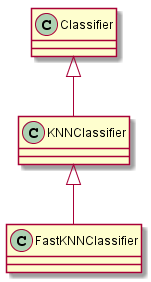
\includegraphics[width=0.3\linewidth]{files/classifier.png}
    \caption{Übersicht Klassen in V1A2\textunderscore Classifier.py}
\end{figure}


\subsubsection{Betrachtung der Basis-Klasse \textit{Classifier}}

\textit{\textunderscore\textunderscore init\textunderscore\textunderscore(self, C):} Ist der Konstruktor der Klasse

\noindent
\textit{fit(self, X, T)} prüft, ob die Matrizen \textit{X(Trainingsdaten)} und \textit{T(Klassenlabels)} die richtigen Dimensionen haben und speichert die Anzahl der Labels in \textit{self.C}.

\noindent
\textit{predict(self, x):} Abstrakte Methode, die von den abgeleiteten Klassen implementiert werden muss, um die naheliegenste Klasse herauszufinden.

\noindent
\textit{crossvalidate(self, S, X, T):} Berechnet die Verwechslungsmatrix und
die Chance für einen Klassifizierungsfehler.

\subsection{Die Klasse \textit{KNNClassifier}}

\subsubsection{Wie lernt ein k-NN-Klassifikator?}

Der k-NN Klassifikator bestimmt die euklidische Distanz der k nächsten, bereits klassifizierten Nachbarn zu einem Merkmalsvektor.  Der Merkmalsvektor wird der Klasse zugewiesen, welche unter der k Nachbarn am häufigsten vorkommt. 

\vspace{5px}
\noindent
\noindent
\textit{fit(self, X, T):} Ruft die fit-Methode der Basisklasse auf. Wenn korrekt, weist diese Methode die Matrizen X und T den Klassenattributen zu.

\subsubsection{
    Implementierung der Methode \textit{getKNearestNeighbors(self, x, k=None, X=None)}
    }

\begin{figure}[H]
    \centering
    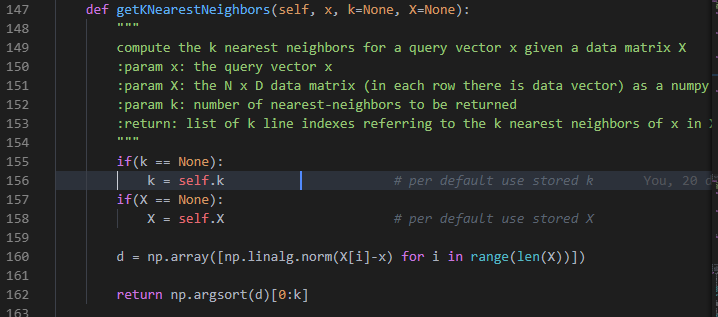
\includegraphics[width=1\linewidth]{files/aufgabe2b2.png}
    \caption{Implementierung}
\end{figure}

\subsubsection{Implementierung der Methode \textit{predict(self, x, k=None)}}

\begin{figure}[H]
    \centering
    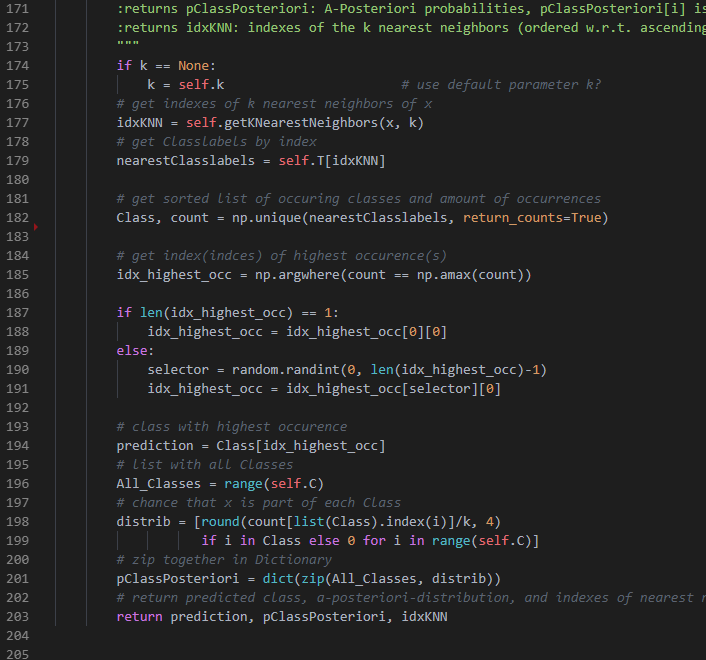
\includegraphics[width=1\linewidth]{files/aufgabe2b3.png}
    \caption{Implementierung}
\end{figure}

\subsection{Test der vollständig implementierten Klasse KNNClassifier}

\subsubsection{Ergebnisse der Tests}

\begin{figure}[H]
    \centering
    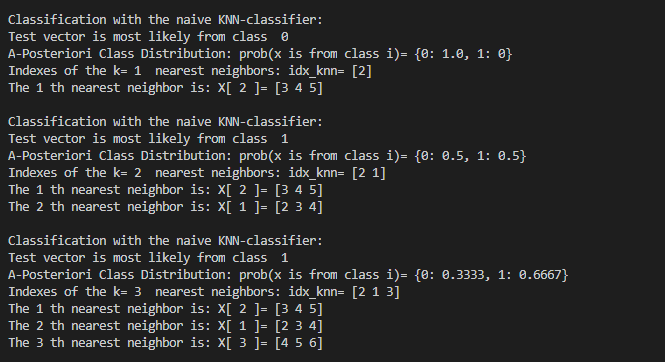
\includegraphics[width=1\linewidth]{files/aufgabe2c.png}
    \caption{Testergebnisse}
\end{figure}

\subsubsection{Warum sollte man für C = 2 Klassen immer ungerades k wählen?}

Da wenn man bei C = 2 z. B. k = 2 wählt, es sein kann, dass einer der Nachbarn Label 0 und der andere Label 1 hat und der Merkmalsvektor somit beiden Klassen zu 50\% zugeordnet wird. Bei ungeradem k wird somit eine klare Klassentrennung
gewährleistet.

\subsection{Vervollständigung der von \textit{KNNClassifier} abgeleiteten Klasse \textit{FastKNNClassifier}}

\subsubsection{Die Methode \textit{fit(self, X, T)}}

\begin{figure}[H]
    \centering
    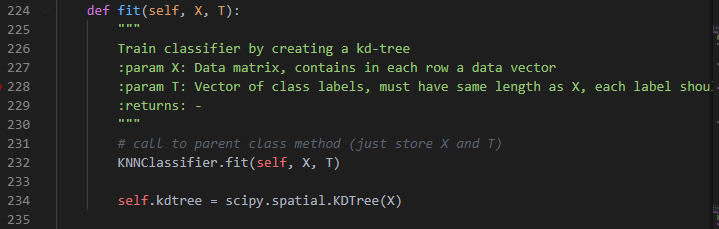
\includegraphics[width=1\linewidth]{files/aufgabe2d1.png}
    \caption{Implementierung}
\end{figure}

\subsubsection{Die Methode \textit{getKNearestNeighbors(self, x, k=None)}}

\begin{figure}[H]
    \centering
    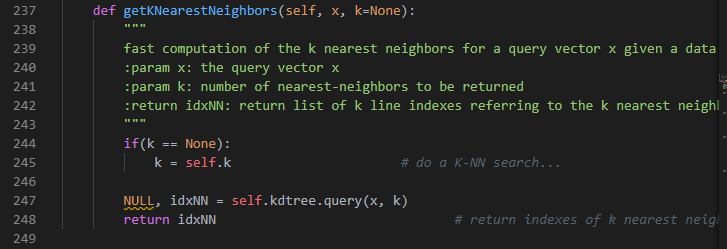
\includegraphics[width=1\linewidth]{files/aufgabe2d2.png}
    \caption{Implementierung}
\end{figure}

\subsubsection{Test der Klasse \textit{FastKNNClassifier}}

\begin{figure}[H]
    \centering
    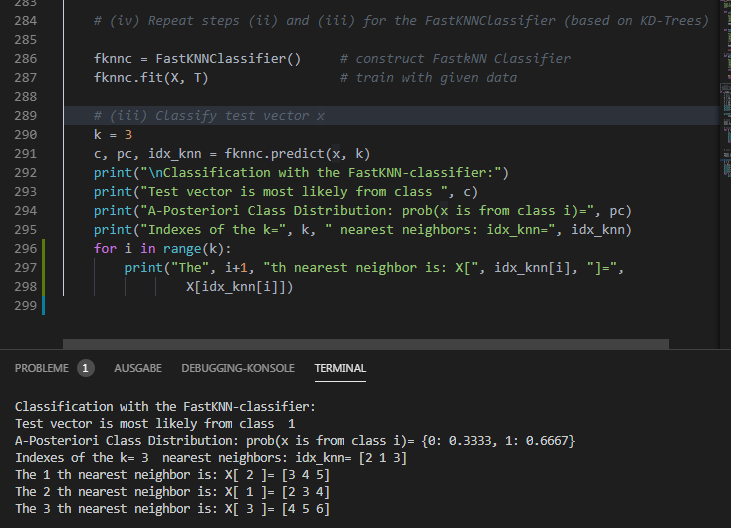
\includegraphics[width=1\linewidth]{files/aufgabe2d3.png}
    \caption{Testergebnisse}
\end{figure}